%\documentclass[11pt,a4paper]{article}
%\usepackage{fullpage}
%\usepackage{beamerarticle}
%\documentclass[handout,xcolor=pdftex,dvipsnames,table]{beamer}
\documentclass[hyperref={unicode=true}]{beamer}
%\documentclass{article}
%\usepackage{beamerarticle}

%\usepackage{pdfpages} 
%\pdfpagesuselayout{resize}[a4paper,border shrink=5mm,landscape] 

\usepackage[utf8]{inputenc}
\usepackage[english,russian]{babel}
\usepackage{../clrscode3e} 
\usepackage{xcolor}
\usepackage{pstricks, pst-tree, pst-node}


%\usepackage{beamerthemesplit}
\usetheme{default}

\AtBeginSubsection[]
{
  \begin{frame}<beamer>{Раздел}
    \tableofcontents[currentsection,currentsubsection]
  \end{frame}
}

\newtheorem{rtheorem}{Теорема} 
%default}
%themesplit}

\title{Сбалансированные деревья}
\subtitle{Дискретный анализ 2012/13}
\author{Андрей Калинин, Татьяна Романова}
\date{17 сентября 2012\,г. }
\usetheme{default}
%\usefonttheme{serif}
\usefonttheme[onlymath]{serif}
%\usefonttheme{professionalfonts}
%\usetheme{default} 


\begin{document}


\psset{levelsep=1cm, treesep=1cm, linewidth=0.5pt, levelsep=30pt}
\newcommand{\tnd}[1]{\Tcircle{\makebox[5mm][c]{#1}}}
\newcommand{\nilnd} {\Tp[edge=none]}
\newcommand{\rednd}[1]{\Tcircle[linecolor=red!30, %
    fillstyle=solid, fillcolor=red!30] {\makebox[5mm][c]{#1}}}
\newcommand{\blacknd}[1]{\Tcircle[linecolor=black!20, %
    fillstyle=solid, fillcolor=black!20]{\makebox[5mm][c]{#1}}}

\frame {\titlepage}


\frame
{
  \frametitle{Литература}

  \begin{itemize}
  \item Д. Кнут. Искусство программирования, том 3, Сортировка и поиск, 2-е издание,
  М.:Вильямс, 2003, стр. 492--509, п.\,6.2.3. <<Сбалансированные деревья>>.
  \item  Кормен Т., Лейзерсон Ч., Ривест Р., Штайн К.. Алгоритмы:
    построение и анализ, 2-е издание, М.:Вильямс, 2005, стр. 336-359, глава 13,
    <<Красно-черные деревья>>. 
  \end{itemize}
}

\frame{\tableofcontents}

\section{Поиск}

\subsection{Различные подходы}

\frame{
  \frametitle{Где, что и как ищем}
  \begin{itemize}
    \item Храним пары ключ-значение. Хотим найти значения или просто
      факт наличия для ... 
      \begin{itemize}
        \item Точных значений ключей. 
        \item Ключей в интервалах. 
        \item Префиксов ключей. 
        \item Ключей с подстроками. 
        \item Ключей, удовлетворяющих маскам. 
      \end{itemize}
    \item Какова скорость доступа к данным?
      \begin{itemize}
      \item Равномерный (случайный) доступ. 
      \item Скорость неравномерна, есть локальность доступа. 
      \end{itemize}
    \item Как часто ... 
      \begin{itemize}
        \item Ищем?
        \item Добавляем?
        \item Изменяем?
        \item Удаляем?
      \end{itemize}
  \end{itemize}
}

\frame
{
  \frametitle{Поиск}
  \begin{itemize}
    \item Основные алгоритмы:
  \begin{itemize}
    \item Последовательный поиск --- $O(n)$.
    \item Бинарный поиск в статическом отсортированном массиве~--- $O(\log n)$.
    \item Поиск в сбалансированных и сильноветвящихся деревьях~---  $O(\log n)$.
    \item Поиск с использованием хеширования ---  $O(1)$ при наличии <<хорошей>> хеш-функции.
    \item Цифровой поиск. Время работы $O(|key|)$.
  \end{itemize}
  \item Специализированные алгоритмы:
  \begin{itemize}
    \item Оптимальные деревья поиска. 
    \item String B-tree.
    \item Суффиксные деревья. 
  \end{itemize}
\end{itemize}
}

\frame{
  \frametitle{Дерево поиска}
  \begin{itemize}
    \item Левое поддерево содержит меньшие ключи, правое --- большие. 
    \item Может выродиться в линейный список. 
    \item Идеально сбалансированное дерево поиска --- дерево наименьшей
      высоты ($\log_2 n$).
    \item Сбалансированное дерево --- дерево, для которого выполняется
      какое-то условие баланса. 
  \end{itemize}
}


\section{AVL-деревья}
\subsection{Определение, высота дерева}
\frame{
  \frametitle{AVL-деревья}
  \begin{itemize}
  \item Обычное дерево поиска при <<плохих>> данных вырождается в линейный список. 
  \item Высота дерева --- длина самого длинного пути от корня к листу.
  \item AVL-дерево --- это то, у которого высота левого поддерева любого узла отличается от высоты правого не более, чем на 1.
  \item Удаление, добавление и поиск элемента в AVL-дереве производится за $O(\log n)$.
  \end{itemize}
}



\frame {
  \frametitle{Минимальное AVL-дерево}

  \begin{center}
  \pstree{\tnd{8}} {
    \pstree{\tnd{5}} {
      \pstree{\tnd{3}} {
        \pstree{\tnd{2}}{\tnd{1} \nilnd}
        \tnd{4}
      }
      \pstree{\tnd{7}}{\tnd{6} \nilnd}  
    }
    \pstree{\tnd{11}}{
      \pstree{\tnd{10}}{\tnd{9} \nilnd}
      \tnd{12}
    }
  }
  \end{center}
}

\frame {
  \frametitle{Высота AVL-дерева}
 \begin{rtheorem}
  Высота AVL-дерева есть $O(\log n)$, где $n$ --- количество узлов в дереве. 
  \end{rtheorem}
  \begin{proof}
  Пусть $T_h$ --- минимальное AVL-дерево. Высота одного из его поддеревьев (например, левого) равна $h - 1$, другого --- $h - 2$. Высоты поддеревьев $T_{h-1}$ будут равны $h-2$ и $h-3$ и т.\,п.

  $n_{min} = 1 + 1 + 2 + \dots + F_{h}$, где $F_{h}$ --- $h$-е число Фибоначчи.
  $n \ge \sum_{i=1}^h F_{i} = F_{i+2} - 1 \sim \phi^{h+2} / \sqrt{5}$.


  $h = O(\log n)$.
  \end{proof}
}

\subsection{Вставка}
\frame {
  \frametitle{Вставка в AVL-дерево}
  \begin{enumerate}
  \item Поиск ключа в дереве. 
  \item Вставка нового ключа. 
  \item Перебалансировка дерева при необходимости:
    \begin{enumerate}
    \item Перевычисляем баланс по пути наверх. 
    \item Если баланс нарушен, выполняем один из поворотов. 
  \end{enumerate}
 \end{enumerate}
}

\frame{
  \frametitle{Балансировка при вставке}
  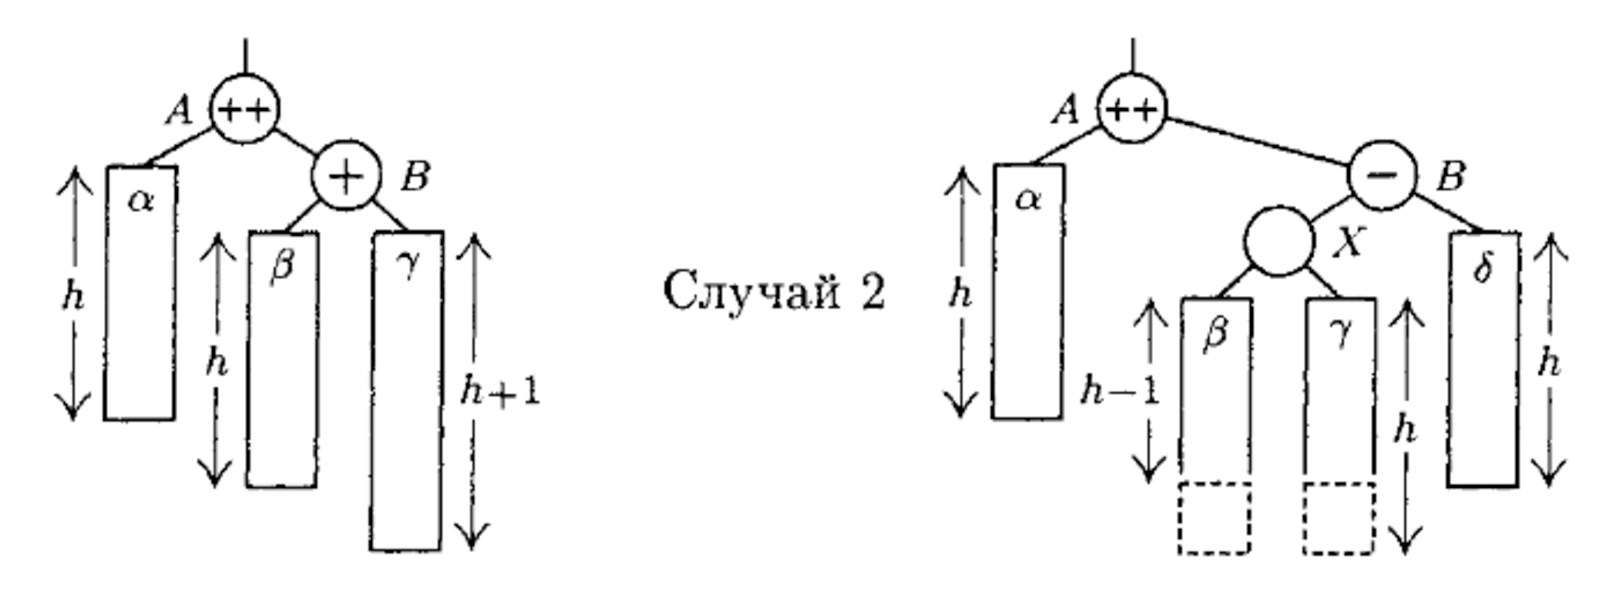
\includegraphics[width=\textwidth]{avl-disbalance.eps}\\
  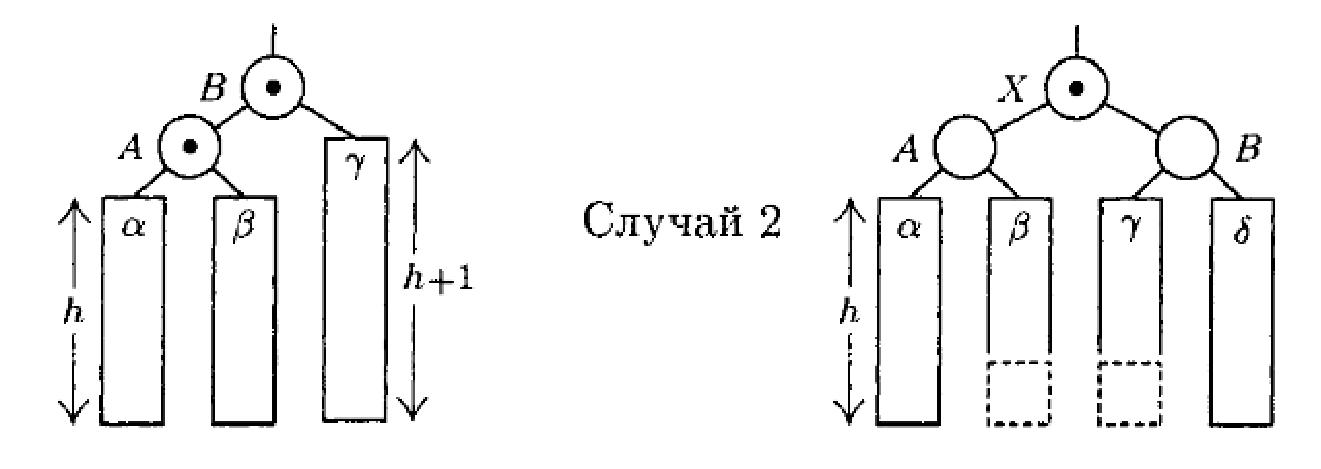
\includegraphics[width=\textwidth]{avl-rebalance.eps}
}

\subsection{Удаление}
\frame {
  \frametitle {Удаление из AVL-дерева}
  \begin{itemize}
  \item Найти узел $X$ с ключом, который нужно удалить.
  \item Если $X.r = NIL$ или $X.l = NIL$, то $R = X$, иначе найти узел $Y$, следующий по порядку за узлом $X$ (самый левый в правом поддереве) и заместить ключ в $X$ ключом в $Y$ и $R = Y$.

$P_0 = head, D_0 = +1, link(D_i, P_i) = P_{i+1}$,
  \item При поиске узла $R$ класть в стек пары $(P_k, D_k)$, $k = 0 \dots l$. 

$P_l = R, link(D_l, P_l) = NIL$.
  \item $link(D_{l-1}, P_{l-1}) = link(-D_l, P_l)$.
  \item Скорректировать фактор сбалансированности $P_{l-1}$.

  \end{itemize}
}

\frame {
  \frametitle {Корректировка баланса $P_k$}
  \begin{itemize}
  \item Если $k = 0$, завершить выполнение алгоритма.
  \item $bal(P_k) = D_k \Longrightarrow bal(P_k) \gets 0, k \gets k-1$, повторить корректировку для нового $k$.
  \item $bal(P_k) = 0 \Longrightarrow bal(P_k) \gets -D_k$, завершить выполнение алгоритма.
  \item $bal(P_k) = -D_k \Longrightarrow $ требуется перебалансировка:
    \begin{itemize}
      \item Аналогично добавлению: рассматриваем поддерево, в котором
        не удаляли элемент, как дерево с добавленным элементом. 
      \item Добавляется третий случай, аналогичный первому но с
        высотой $\beta$ равной $h+1$.
    \end{itemize}
  \item Важное отличие от добавления элемента: может потребоваться
    $\log n$ поворотов, тогда как для добавления не требуется больше 1.
  \end{itemize}
}

\section{Красно-черные деревья}
\subsection{Определение, высота дерева}
\frame {
  \frametitle {Красно-черные деревья}
  \begin{enumerate}
    \item Каждый узел является либо красным либо черным.
    \item Корень дерева является черным.
    \item Каждый лист дерева (NIL) является черным.
    \item Если узел дерева красный, то оба дочерних узла --- черные.
    \item Для каждого узла все пути от него до листьев-потомков содержат одинаковое количество черных узлов.
  \end{enumerate}
}

\psset{levelsep=1cm, treesep=0.5cm, linewidth=0.5pt, levelsep=30pt}
\frame {
  \frametitle {Пример}
  \begin{center}
  \pstree{\blacknd{26}} {
    \pstree{\rednd{17}} {
      \pstree{\blacknd{14}} {
        \pstree{\rednd{10}} {
          \pstree{\blacknd{7}}{\rednd{3} \nilnd}
          \blacknd{12}
        }
        \pstree{\blacknd{16}}{\rednd{15} \nilnd}
      }
      \pstree{\blacknd{21}} {
        \pstree{\blacknd{19}}{\nilnd \rednd{20}}
        \blacknd{23}
      }
    }
    \pstree{\blacknd{41}} {
      \pstree{\rednd{30}} {
        \blacknd{28}
        \pstree{\blacknd{38}}{\rednd{35} \rednd{39}}
      }
      \blacknd{47}
    }
  }
  \end{center}
}

\frame {
  \frametitle {Высота красно-черного дерева}
 \begin{rtheorem}
    Красно-чёрное дерево с $n$ внутренними узлами имеет высоту не
    более чем $2 \log_2(n+1)$.
  \end{rtheorem}
  \begin{proof}
  \begin{enumerate}
    \item $bh(x)$ --- черная высота узла $x$ (количество черных узлов на пути от $x$ к листу, не считая x).
    \item Максимальная и минимальная высоты поддеревьев отличаются не больше, чем в 2 раза (из свойств 4 и 5).
    \item Минимальное красно-черное дерево состоит только из черных узлов.

        Следовательно, $n \ge 2^{h_{min}} - 1$,
        
        $h_{max} = 2 h_{min} \le 2\log_2(n+1)$
    \item Вывод: высота красно-черного дерева $h = O(\log n)$.
  \end{enumerate}
  \end{proof}
}

\subsection{Вставка}
\psset{treesep=1.5cm, levelsep=16pt}

\frame
{
  \frametitle{Вставка. Иллюстрация}
  \begin{center}
  \pstree {\blacknd{11}}{
    \pstree{\rednd{2}}{
      \blacknd{1} 
      \pstree{\blacknd{7}}{
        \pstree{\rednd{5}}{\rednd{4,z} \nilnd}
        \rednd{8,y}
      }
    }
    \pstree{\blacknd{14}}{\nilnd \rednd{15}}
  }

  \pstree {\blacknd{11}}{
    \pstree{\rednd{2}}{
      \blacknd{1} 
      \pstree{\rednd{7,z}}{
        \pstree{\blacknd{5}}{\rednd{4} \nilnd}
        \blacknd{8}
      }
    }
    \pstree{\blacknd{14,y}}{\nilnd \rednd{15}}
  }
  \end{center}
}

\frame {
  \frametitle{Вставка. Иллюстрация}
  \begin{center}
   \pstree {\blacknd{11}}{
    \pstree{\rednd{7}}{
      \pstree{\rednd{2,z}}{
        \blacknd{1}
        \pstree{\blacknd{5}}{\rednd{4} \nilnd}
      }
      \blacknd{8}
    }
    \pstree{\blacknd{14,y}}{\nilnd \rednd{15}}
  }

  \pstree {\blacknd{7}}{
    \pstree{\rednd{2}}{
      \blacknd{1}
      \pstree{\blacknd{5}}{\rednd{4} \nilnd}
    }
    \pstree{\rednd{11}}{
      \blacknd{8}
      \pstree{\blacknd{14}}{\nilnd \rednd{15}}
    }
  }
  \end{center}
}


\frame
{
  \frametitle{Вставка. Общая идея}
  \begin{itemize}
    \item Выполняется вставка узла $z$ в дерево $T$ (как в обычное дерево поиска).
    \item Вставленный узел красится в красный цвет, $color(z) = red$. Возможно нарушено свойство 4.
    \item Вызывается процедура, гарантирующая корректность нового дерева. До тех пор, пока родитель узла $z$ красный:
      \begin{itemize}
        \item Пусть $y$ --- <<дядя>> узла $z$, если дядя красный, то нужно перекрасить его и отца в черный цвет, а дедушку в красный, и переместить указатель $z$ на дедушку.
        \item Если дядя черный, а узел $z$ --- левый сын, то нужно повернуть вправо отца и деда, отца покрасить в черный, деда в красный (у него гарантированно 2 черных сына).
        \item Если дядя черный, а узел $z$ --- правый сын, то нужно повернуть $z$ и отца влево и переместить указатель $z$ на бывшего отца $z$. Задача свелась к предыдущей.
      \end{itemize}
  \end{itemize}
}

\frame
{
  \frametitle{Вставка. Алгоритм}
  \begin{codebox}
    \Procname{$\proc{RB-Insert-Fixup}(T, z)$}
      \li \While $color[p[z]] = RED$ 
      \li \Do \If $p[z] = left[p[p[z]]]$
      \li \Then $y := right[p[p[z]]]$
      \li \If $color[y] = RED$
      \li \Then $color[p[z]] :=  color[y] := BLACK$ 
      \li       $color[p[p[z]]] := RED$, $z := p[p[z]]$       
      \li \Else \If $z = right[p[z]]$
      \li   \Then $\proc{Left-Rotate}(z, p[z])$
      \li         $z := left[z]$ \End
      \li   $color[p[z]] := BLACK$, $color[p[p[z]]] := RED$   
      \li   $\proc{Right-Rotate}(p[z], p[p[z]])$ \End
      \li   \Else (то же, с заменой $left$ на $right$ и наоборот) \End \End
      \li $color[root[T]] := BLACK$
  
  \end{codebox}
}

\subsection{Удаление}
\psset{treesep=0.5cm, levelsep=20pt}
\frame
{
  \frametitle{Удаление. Иллюстрация}
  \begin{center}
    \pstree{\blacknd{B}}{
      \pstree{\blacknd{A,x}}{\Tr{$\alpha$} \Tr{$\beta$}} 
      \pstree{\rednd{D,w}}{
        \pstree{\blacknd{C}}{\Tr{$\gamma$} \Tr{$\delta$}}
        \pstree{\blacknd{E}}{\Tr{$\epsilon$} \Tr{$\phi$}}
      }
    }
    ~$\Rightarrow$
    \pstree{\blacknd{D}}{
      \pstree{\rednd{B}}{
        \pstree{\blacknd{A,x}}{\Tr{$\alpha$} \Tr{$\beta$}}
        \pstree{\blacknd{C,w}}{\Tr{$\gamma$} \Tr{$\delta$}}
      }
      \pstree{\blacknd{E}}{\Tr{$\epsilon$} \Tr{$\phi$}} 
    }
\vfill
    \pstree{\tnd{B}}{
      \pstree{\blacknd{A,x}}{\Tr{$\alpha$} \Tr{$\beta$}} 
      \pstree{\blacknd{D,w}}{
        \pstree{\blacknd{C}}{\Tr{$\gamma$} \Tr{$\delta$}}
        \pstree{\blacknd{E}}{\Tr{$\epsilon$} \Tr{$\phi$}}
      }
    }
    ~$\Rightarrow$
    \pstree{\tnd{B, x}}{
      \pstree{\blacknd{A}}{\Tr{$\alpha$} \Tr{$\beta$}} 
      \pstree{\rednd{D,w}}{
        \pstree{\blacknd{C}}{\Tr{$\gamma$} \Tr{$\delta$}}
        \pstree{\blacknd{E}}{\Tr{$\epsilon$} \Tr{$\phi$}}
      }
    }  
  \end{center}
}

\frame
{
  \frametitle{Удаление. Иллюстрация}
  \begin{center}
    \pstree{\tnd{B}}{
      \pstree{\blacknd{A,x}}{\Tr{$\alpha$} \Tr{$\beta$}} 
      \pstree{\blacknd{D,w}}{
        \pstree{\rednd{C}}{\Tr{$\gamma$} \Tr{$\delta$}}
        \pstree{\blacknd{E}}{\Tr{$\epsilon$} \Tr{$\phi$}}
      }
    }
    ~$\Rightarrow$
    \pstree{\tnd{B}}{
      \pstree{\blacknd{A,x}}{\Tr{$\alpha$} \Tr{$\beta$}} 
      \pstree{\blacknd{C,w}}{
        \Tr{$\gamma$}
        \pstree{\rednd{D}} {
          \Tr{$\delta$}
          \pstree{\blacknd{E}}{\Tr{$\epsilon$} \Tr{$\phi$}}
        }
      }
    }
\vfill
    \pstree{\tnd{B}}{
      \pstree{\blacknd{A,x}}{\Tr{$\alpha$} \Tr{$\beta$}} 
      \pstree{\blacknd{D,w}}{
        \pstree{\tnd{C}}{\Tr{$\gamma$} \Tr{$\delta$}}
        \pstree{\rednd{E}}{\Tr{$\epsilon$} \Tr{$\phi$}}
      }
    }
    ~$\Rightarrow$
    \pstree{\tnd{D}}{
      \pstree{\blacknd{B}} {
        \pstree{\blacknd{A}}{\Tr{$\alpha$} \Tr{$\beta$}} 
        \pstree{\tnd{C}}{\Tr{$\gamma$} \Tr{$\delta$}}
      }

      \pstree{\blacknd{E}}{\Tr{$\epsilon$} \Tr{$\phi$}}
    }  
  \end{center}
}

\frame
{
  \frametitle{Удаление. Общая идея}
  \begin{itemize}
    \item Выполняется удаление узла $z$ из дерева $T$ (как из обычного дерево поиска).
    \item Если у узла $z$ есть оба сына, то находится узел $y$ --- следующий по порядку, у которого нет одного из сыновей.
    \item Существующего сына узла $y$ (или $z$) назовем $x$.
    \item Если удалялся черный узел, то оказалось нарушено свойство 5.
    \item Вызывается процедура, гарантирующая корректность нового дерева. До тех пор, пока $x$ не корень, и пока он черный (если $x$ --- красный, то можно перекрасить его, и дерево станет корректным), выполнять некоторые действия.
  \end{itemize}
}

\frame
{
  \frametitle{Удаление. Алгоритм}
  \begin{codebox}
    \Procname{$\proc{RB-Delete-Fixup}(T, x)$}
      \li \While $x \ne root[T]$ и $color[x] = BLACK$ 
      \li \Do \If $x = left[p[x]]$
      \li \Then $w := right[p[x]]$
      \li \If $color[w] = RED$
      \li \Then $color[w] :=  BLACK, color[p[x]] := RED$ 
      \li       $\proc{Left-Rotate}(w, p[x])$
      \li       $w := right[p[x]]$ \End
      \li \If $color[left[w]] = BLACK$ и $color[right[w]] = BLACK$
      \li   \Then $color[w] := RED$
      \li         $x := p[x]$ \End
  
  \end{codebox}
}

\frame
{
  \frametitle{Удаление. Алгоритм}
  \begin{codebox}
    \Procname{$\proc{RB-Delete-Fixup}(T, x)$}
      \li \While $x \ne root[T]$ и $color[x] = BLACK$ 
      \li \Do \If $x = left[p[x]]$
      \li \Then \Else \If $color[right[w]] = BLACK$
      \li \Then $color[left[w]] :=  BLACK, color[w] := RED$ 
      \li       $\proc{Right-Rotate}(left[w], w)$
      \li       $w := right[p[x]]$ \End
      \li   $color[w] := color[p[x]]$
      \li   $color[p[x]] := BLACK$
      \li   $color[right[w]] := BLACK$
      \li   $\proc{Left-Rotate}(w, p[x])$
      \li   $x := root[T]$
      \li   \Else (то же, с заменой $left$ на $right$ и наоборот) \End \End
      \li $color[x] := BLACK$
  
  \end{codebox}
}
\end{document}
